%%----------------------------------------------------------------------------
%% Onderzoekstechnieken: Analyse van 2 kwalitatieve variabelen
%%----------------------------------------------------------------------------

\documentclass[aspectratio=169]{beamer}

%==============================================================================
% Aanloop
%==============================================================================

%---------- Vormgeving --------------------------------------------------------

\usetheme{hogent}

\usecolortheme{hgwhite} % witte achtergrond, zwarte tekst

\usepackage{graphicx,multicol}
\usepackage{comment,enumerate,hyperref}
\usepackage{amsmath,amsfonts,amssymb}
\usepackage[dutch]{babel}
\usepackage{multirow}
\usepackage{eurosym}
\usepackage{listings}
\usepackage{textcomp}
\usepackage{framed}
\usepackage{wrapfig}
\usepackage{tabu} %needed for \tabulinesep
\usepackage{wrapfig}
\usepackage{pgf-pie}
\usepackage{pgfplots}
\usepackage{booktabs}
\usepackage{pgfplotstable}
\usepackage{changepage}
\usepackage{ulem} % for \sout{text} (strikethrough)
\usepackage{fancyvrb} % for \begin{Verbatim} (LaTeX controls within verbatim)

%---------- Configuratie ------------------------------------------------------

\pgfplotsset{compat=1.16}
\usetikzlibrary{arrows,shapes,backgrounds,positioning,shadows}
\usetikzlibrary{pgfplots.statistics}

%---------- Commando-definities -----------------------------------------------

\newcommand{\tabitem}{~~\llap{\textbullet}~~}
\newcommand{\alertbox}[2][hgblue]{%
  \setbeamercolor{alertbox}{bg=#1,fg=white}
  \begin{beamercolorbox}[sep=2pt,center]{alertbox}
    \textbf{#2}
  \end{beamercolorbox}
}
\pgfmathdeclarefunction{gauss}{2}{%
  \pgfmathparse{1/(#2*sqrt(2*pi))*exp(-((x-#1)^2)/(2*#2^2))}%
}

%---------- Info over de presentatie ------------------------------------------

\title[OZT: aan de slag]{Hst 6. Analyse van 2 (kwalitatieve) variabelen}
\subtitle{Onderzoekstechnieken}
\author{Jens Buysse \and Wim {De Bruyn} \and Pieter-Jan Maenhout \and Bert {Van Vreckem}}
\date{AJ 2019-2020}


%==============================================================================
% Inhoud presentatie
%==============================================================================

\begin{document}

\begin{frame}
  \maketitle
\end{frame}

\begin{frame}
  \frametitle{What's on the menu today?}
  
  \tableofcontents
\end{frame}

\begin{frame}
  \frametitle{Leerdoelen}
  
  \begin{itemize}
    \item Afhankelijke/onafhankelijke variabele
    \item Voor elk meetniveau geschikte analysetechnieken kunnen toepassen
    \item Kruistabellen en Cramér's $V$
    \item Visualisatie
  \end{itemize}
\end{frame}

\begin{frame}
  \frametitle{Overzicht}
    \centering
    \begin{tabular}{lll}
    	\toprule
    	\textbf{Onafhankelijke} & \textbf{Afhankelijke} & \textbf{Toets/metriek}        \\
    	\midrule
    	Kwalitatief             & Kwalitatief           & $\chi^2$-toets                \\
    	                        &                       & Cramér's $V$                  \\
    	Kwalitatief             & Kwantitatief          & $t$-toets voor 2 steekproeven \\
    	                        &                       & Cohen's $d$                   \\
    	Kwantitatief            & Kwantitatief          & ---                           \\
    	                        &                       & Regressie, correlatie         \\
    	\bottomrule
    \end{tabular}
\end{frame}

\section{Bivariate analyse}

\begin{frame}
  \frametitle{Bivariate Analyse}
  \note{Deze slide wordt gebruikt om een voorbeeld te geven van een minder triviaal verband tussen variabelen: Ant Colony optimization. Verbanden tussen variabelen zouden dus kunnen zijn:
    
    \begin{itemize}
      \item Aantal obstakels tussen nest en voedeselbron
      \item Algoritme gebruikt om feromonen weg te nemen / te plaatsen
      \item Vorm van de obstakels tussen nest en voedselbron
      \item \dots
  \end{itemize}}
  \begin{figure}
    \centering
    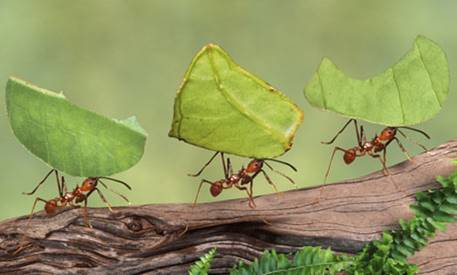
\includegraphics[width=0.8\textwidth]{ants.jpg}
    \label{fig:ants}
  \end{figure}
  
\end{frame}

\begin{frame}
  \frametitle{Voorbeeld}
  \framesubtitle{Tevredenheidsonderzoek campusrestaurant}
  
  \begin{itemize}
    \item Hoe vaakt bezoekt men het restaurant?
    \item Is er een verschil in uitgaven tussen student en medewerker?
    \item Is er een verband tussen het aantal dagen dat men bezoekt en bedrag dat men wekelijks besteedt?
  \end{itemize}
  
  R Code: zie \texttt{cursus/data/catering\_hogeschool.R}
  
  \centering
  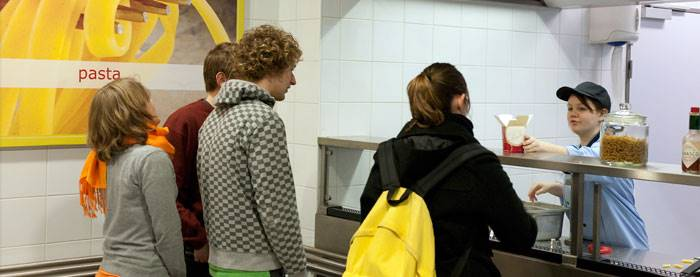
\includegraphics[height=.4\textheight]{students.jpg}
\end{frame}

\begin{frame}{Hoe vaakt bezoekt men het restaurant?}
  \begin{columns}
    \begin{column}{0.5\textwidth}
      \begin{table}[h]
        \small
        \begin{tabular}{|l|l|}
          \hline
          { \textbf{Statistiek}} & \textbf{Waarde} \\ \hline
          Mean                   & 2.96            \\ \hline
          Median                 & 3               \\ \hline
          Mode                   & 2               \\ \hline
          Stdev                  & 1.484           \\ \hline
          Variantie              & 2.202           \\ \hline
          Range                  & 4               \\ \hline
          $Q_{1}$                & 2               \\ \hline
          $Q_{2}$                & 3               \\ \hline
          $Q_{3}$                & 5               \\ \hline
        \end{tabular}
      \end{table}
    \end{column}
    \begin{column}{0.5\textwidth}
      
      \begin{figure}
        \centering
        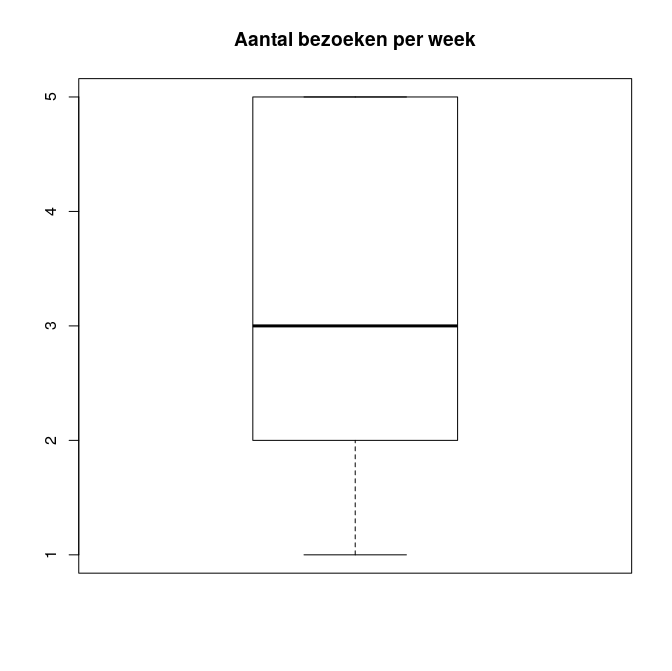
\includegraphics[height=.8\textheight]{2var-boxplot-aantalbezoeken}
        \label{fig:boxplotStudenten}
      \end{figure}
      
    \end{column}
  \end{columns}
\end{frame}

\begin{frame}{Hoe vaakt bezoekt men het restaurant?}
  
  \begin{columns}
    
    \begin{column}{0.5\textwidth}
      \begin{figure}
        \centering
        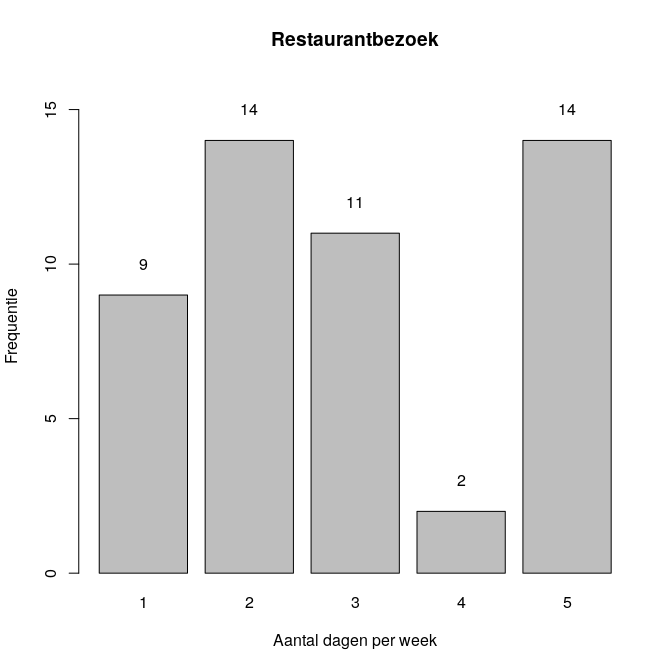
\includegraphics[height=.8\textheight]{2var-barplot-aantalbezoeken}
        \label{fig:studentenbar}
      \end{figure}
    \end{column}
    
    \begin{column}{0.5\textwidth}
      \begin{figure}
        \centering
        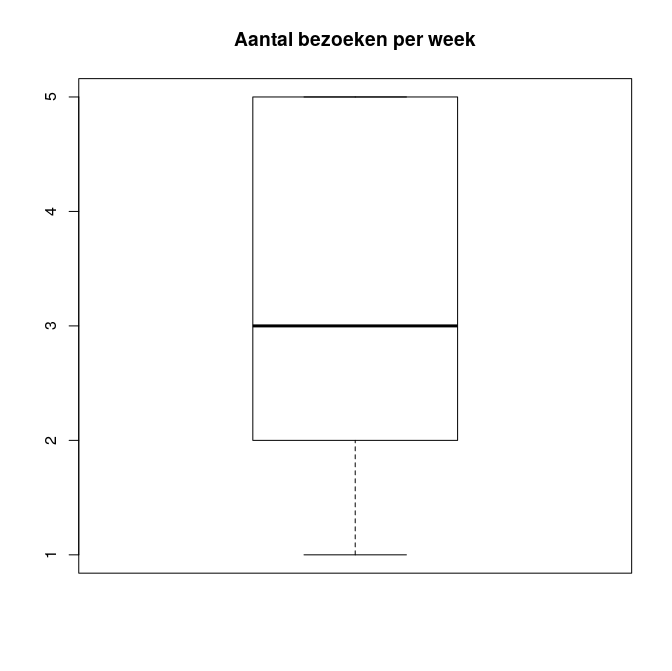
\includegraphics[height=.8\textheight]{2var-boxplot-aantalbezoeken}
        \label{fig:boxplotStudenten2}
      \end{figure}
    \end{column}
    
  \end{columns}
\end{frame}

\begin{frame}{Student vs werknemer}
  
  \begin{itemize}
    \item \alert<1>{Enkelvoudig staafdiagram} (van gemiddelde per categorie)
    \item \alert<2>{Boxplot}
  \end{itemize}
  
  \begin{figure}
    \centering
    \only<1>{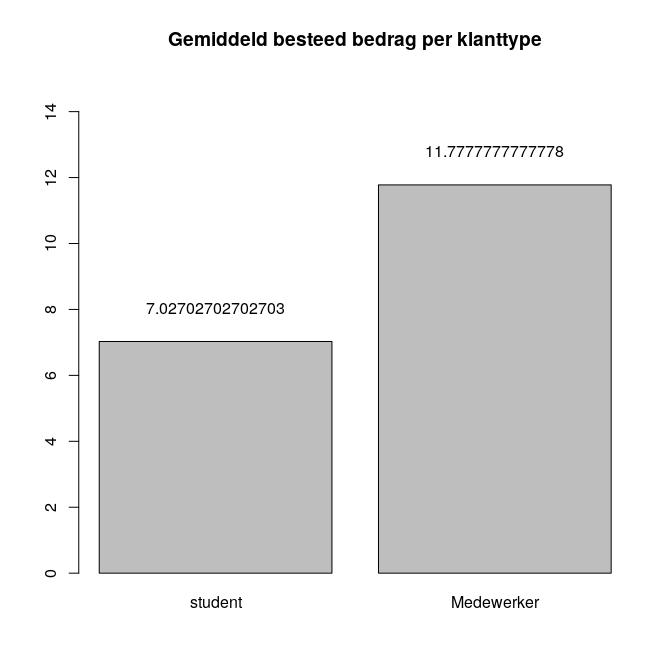
\includegraphics[height=0.6\textheight]{2var-barplot-gemiddeld-bedrag}}
    \only<2>{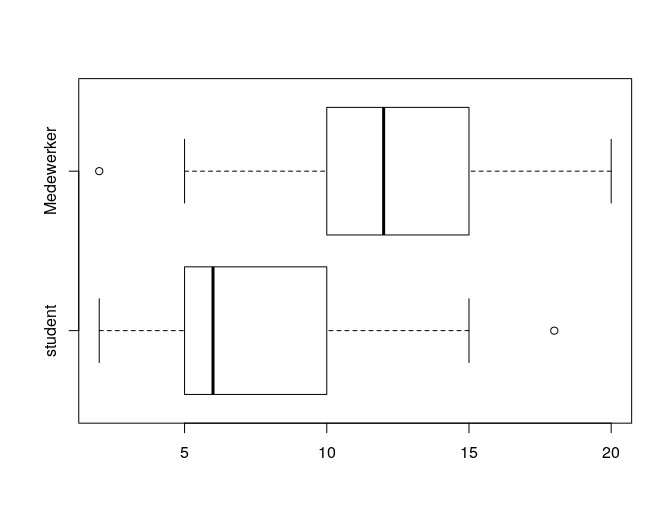
\includegraphics[height=0.6\textheight]{2var-boxplot-klanttype-bedrag}}
  \end{figure}
  
  \only<1>{\textbf{Let op!} Onvoldoende om significant verschil aan te tonen!}
\end{frame}

\begin{frame}
  \frametitle{Afhankelijke en onafhankelijke variabele}
  
  \begin{columns}
    \begin{column}{0.3\textwidth}
      
      \begin{figure}
        \centering
        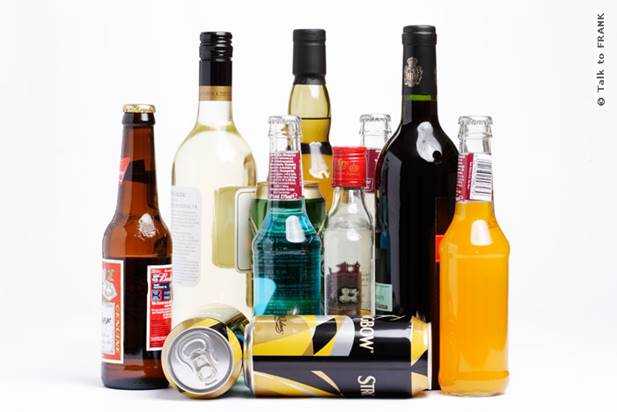
\includegraphics[width=1.00\textwidth]{liquor.jpg}
        \label{fig:liquor}
      \end{figure}
      
    \end{column}
    \begin{column}{0.3\textwidth}
      
      \begin{figure}
        \centering
        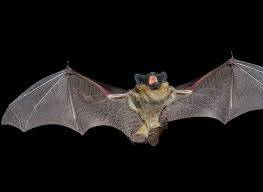
\includegraphics[width=1.00\textwidth]{bat.jpg}
        \label{fig:bat}
      \end{figure}
      
    \end{column}
    \begin{column}{0.3\textwidth}
      
      \begin{figure}
        \centering
        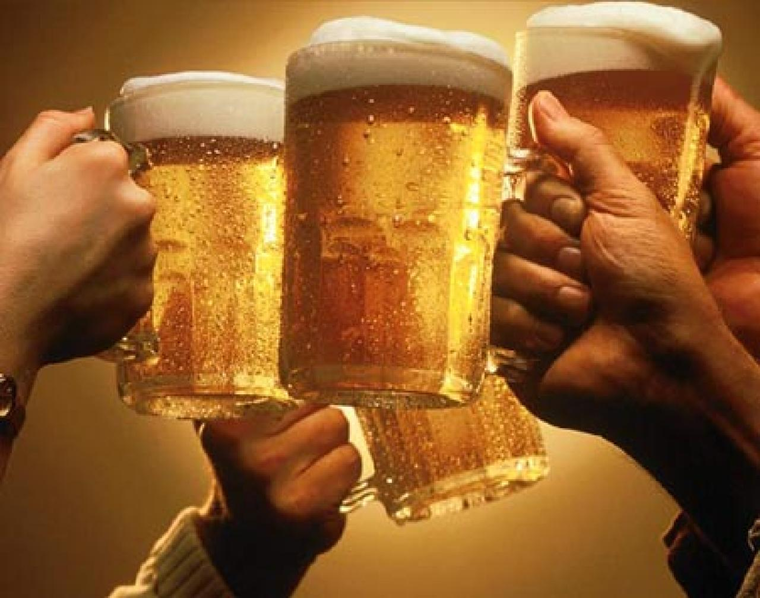
\includegraphics[width=1.00\textwidth]{beer.png}
        \label{fig:beer}
      \end{figure}
      
    \end{column}
  \end{columns}
  \note{Onderzoeken die hier gevoerd zijn:
    
    \begin{itemize}
      \item Invloed van alcoholinname op leervermogen van vleermuizen (Drinking and Flying: Does Alcohol Consumption Affect the Flight and Echolocation Performance of Phyllostomid Bats?)
      \item Arnd Leike of the Ludwig Maximilians University receives one of the Ig Nobel awards - which are given for research that cannot or should not be repeated - for demonstrating that beer froth obeys the mathematical law of exponential decay.
  \end{itemize}}
\end{frame}

\begin{frame}
  \frametitle{Onderzoek academiejaar 2013-2014}
  \begin{columns}
    \begin{column}{0.3\textwidth}
      
      \begin{figure}
        \centering
        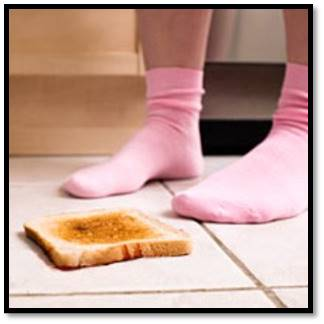
\includegraphics[width=1.00\textwidth]{toast.jpg}
        \label{fig:toast}
      \end{figure}
      
    \end{column}
    \begin{column}{0.3\textwidth}
      
      \begin{figure}
        \centering
        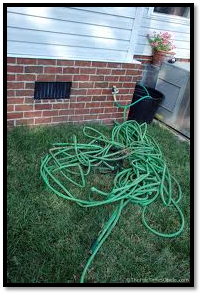
\includegraphics[width=1.00\textwidth]{hose.png}
        \label{fig:hose}
      \end{figure}
      
    \end{column}
    \begin{column}{0.3\textwidth}
      
      \begin{figure}
        \centering
        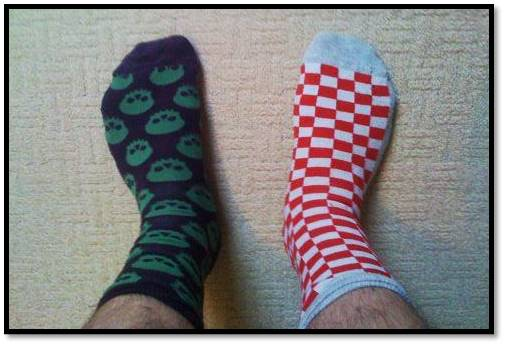
\includegraphics[width=1.00\textwidth]{socks.jpg}
        \label{fig:socks}
      \end{figure}
      
    \end{column}
  \end{columns}
  \note{Studenten moesten onderzoeken of er een verband was tussen vallen van boterham op boterzijde en hoogte e.a., of verband was tussen het aantal onpare sokken en andere fenomenen zoals je eigen was doen, veel sporten al dan niet \dots}
\end{frame}

\section{Kruistabellen en Cramér's V}

\begin{frame}
  \frametitle{Kruistabellen}
  Is er een verschil in waardering in het assortiment tussen mannen en vrouwen?
  
  \begin{table}[h]
    \begin{tabular}{l||l|l||l}
      & Vrouw & Man & Totaal \\ \hline \hline
      Goed        & 9     & 8   & 17     \\
      Voldoende   & 8     & 10  & 18     \\
      Onvoldoende & 5     & 5   & 10     \\
      Slecht      & 0     & 4   & 4      \\ \hline \hline
      Totaal      & 22    & 27  & 49     \\
    \end{tabular}
  \end{table}
\end{frame}

\begin{frame}
  \frametitle{Chi-kwadraat ($\chi^2$) }
  
  \alertbox{Chi-kwadraat ($\chi^2$) is een metriek die aangeeft hoeverre de waarden in een kruistabel afwijken van de verwachte waarden als je veronderstelt dat er \textit{geen} verband is tussen twee variabelen.}
  
  \[ \chi^2 = \sum \frac{(o - e)^2}{e} \]
  
  \begin{itemize}
    \item De som wordt berekend over alle cijfers in een kruistabel
    \item $o$: geobserveerde waarde
    \item $e$: verwachte waarde
  \end{itemize}
\end{frame}

\begin{frame}
  \frametitle{Kruistabellen}
  \framesubtitle{Percenteren}
  
  \begin{adjustwidth}{-1.5em}{-1.5em}
    \begin{table}[h] \centering
      \begin{tabular}{@{}rrrrrrr@{}} \toprule
        & Vrouw & Man & Totaal & Vrouw \% & Man\%   & Totaal  \\ \midrule
        Goed        & $9$     & $8$  & $17$     & $41$\%  & $30$\%  & $35$\% \\
        Voldoende   & $8$     & $10$ & $18$     & $36$\%  & $37$\%  & $37$\% \\
        Onvoldoende & $5$     & $5$  & $10$     & $23$\%  & $18$\%  & $20$\% \\
        Slecht      & $0$     & $4$  & $4$      & $0$\%   & $15$\%  & $8$\%  \\
        Totaal      & $22$    & $27$ & $49$     & $100$\% & $100$\% & $100$\%\\
        \bottomrule
      \end{tabular}
    \end{table}
  \end{adjustwidth}
\end{frame}

\begin{frame}
  \frametitle{Kruistabellen}
  \framesubtitle{Verschil bepalen $(o - e)$}
  
  \begin{adjustwidth}{-1.5em}{-1.5em}
    \begin{table}[h] \centering
      \begin{tabular}{@{}rrrrrrr@{}} \toprule
        & Vrouw & Man & Totaal & Vrouw \% & Man\%   & Totaal  \\ \midrule
        Goed        & $9 -\textcolor{red}{7.63}$     & $8 - \textcolor{red}{9.36}$   & $17$     & $41$\%  & $30$\% & $35$\% \\
        Voldoende   & $8 - \textcolor{red}{8.08}$   & $10 - \textcolor{red}{9.91}$  & $18$     & $36$\%  & $37$\%    & $37$\% \\
        Onvoldoende & $5 - \textcolor{red}{4.48}$    & $5 - \textcolor{red}{5.51}$  & $10$     & $23$\%  & $18$\% & $20$\% \\
        Slecht      & $0 - \textcolor{red}{1.79}$    & $4 - \textcolor{red}{2.20}$  & $4$      & $0$\%      & $15$\% & $8$\%  \\
        Totaal      & $22$    & $27$  & $49$     & $100$\%    & $100$\%   & $100$\%   \\
        \bottomrule
      \end{tabular}
    \end{table}
  \end{adjustwidth}
\end{frame}

\begin{frame}
  \frametitle{Kruistabellen}
  \framesubtitle{Kwadrateren en normaliseren $\frac{(o-e)^2}{e}$}
  
  \begin{table}[h] \centering
    \begin{tabular}{@{}rrrrrrr@{}} \toprule
      & Vrouw                   & Man                     & Totaal & Vrouw \% & Man\%   & Totaal  \\
      \midrule
      Goed        & $\textcolor{blue}{0.2}$ & $\textcolor{blue}{0.2}$ & $17$   & $41$\%   & $30$\%  & $35$\% \\
      Voldoende   & $\textcolor{blue}{0}$   & $\textcolor{blue}{0}$   & $18$   & $36$\%   & $37$\%  & $37$\% \\
      Onvoldoende & $\textcolor{blue}{0.1}$ & $\textcolor{blue}{0}$   & $10$   & $23$\%   & $18$\%  & $20$\% \\
      Slecht      & $\textcolor{blue}{1.8}$ & $\textcolor{blue}{1.5}$ & $4$    & $0$\%    & $15$\%  & $8$\%  \\
      Totaal      & $22$                    & $27$                    & $49$   & $100$\%  & $100$\% & $100$\%   \\
      \bottomrule
    \end{tabular}
  \end{table}
  \[ \chi^{2} = 3.811, V= 0.279 \]
\end{frame}

\begin{frame}
  \frametitle{Cramér's V}
  
  \alertbox{Cramér's V is een maat die aanduidt hoe sterk de samenhang is tussen twee kwalitatieve variabelen. Dit getal ligt altijd tussen 0 en 1}
  
  \[ V = \sqrt{\frac{\chi^2}{n (k - 1)}} \]
  
  $n$: het aantal waarnemingen
  
  $k$: min(aantal rijen, aantal kolommen)
\end{frame}

\begin{frame}
  \frametitle{Interpretatie Cramér's V}
  
  \begin{table}[h] \centering
    \begin{tabular}{@{}rr@{}} \toprule
      Waarde & Interpretatie \\
      \midrule
      $0$ & geen samenhang \\
      $0.1$ &  zwakke samenhang \\
      $0.25$ & redelijk sterke samenhang \\
      $0.5$ & sterke samenhang \\
      $0.75$ & zeer sterke samenhang \\
      $1$ & volledige samenhang \\
      \bottomrule
    \end{tabular}
  \end{table}
\end{frame}

\begin{frame}
  \frametitle{Voorbeeld 2}
  \framesubtitle{Verband tussen geslacht en voorkeur automerk}
  
  \begin{table}[h] \centering
    \begin{tabular}{@{}rrrrrr@{}} \toprule
      & Mercedes & BMW & Porsche& Alfa Romeo & Totaal \\
      \midrule
      Mannen  & $10$ & $10$ & $20$ & $20$ & $60$ \\
      Vrouwen & $20$ & $5$  & $15$ & $0$  & $40$ \\
      Totaal  & $30$ & $15$ & $35$ & $20$ & $100$ \\
      \bottomrule
    \end{tabular}
  \end{table}
  Het lijkt alsof de automerken niet gelijkelijk gewaardeerd worden door mannen en vrouwen.
  \[ \chi^{2} = 22.619, V = \sqrt{\frac{22.169}{100 . (2-1)}}  = 0.476\]
\end{frame}

\section{Grafieken voor kruistabellen}

\begin{frame}
  \frametitle{Visuele voorstelling van kruistabelen}
  
  \begin{figure}
    \centering
    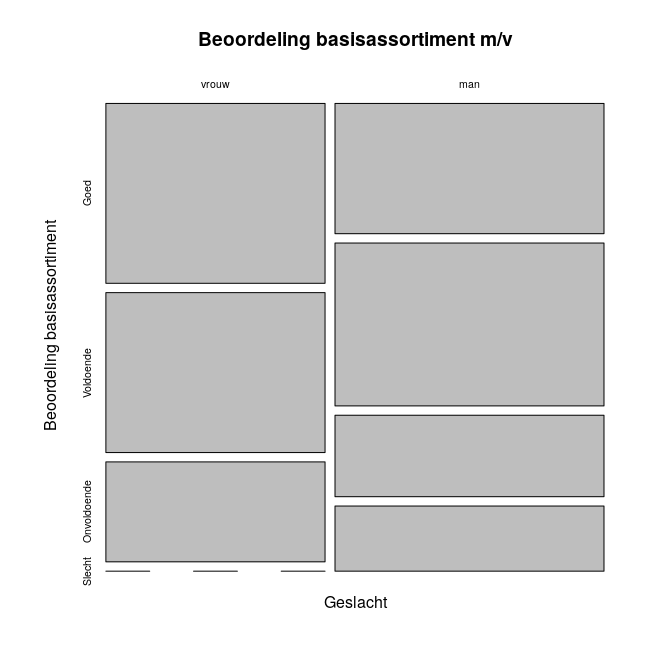
\includegraphics[height=.9\textheight]{2var-xtab-plot-waardering}
  \end{figure}
  
\end{frame}

\begin{frame}
  \frametitle{Visuele voorstelling van kruistabelen}
  \framesubtitle{Geclusterde staafgrafiek}
  
  \begin{figure}
    \centering
    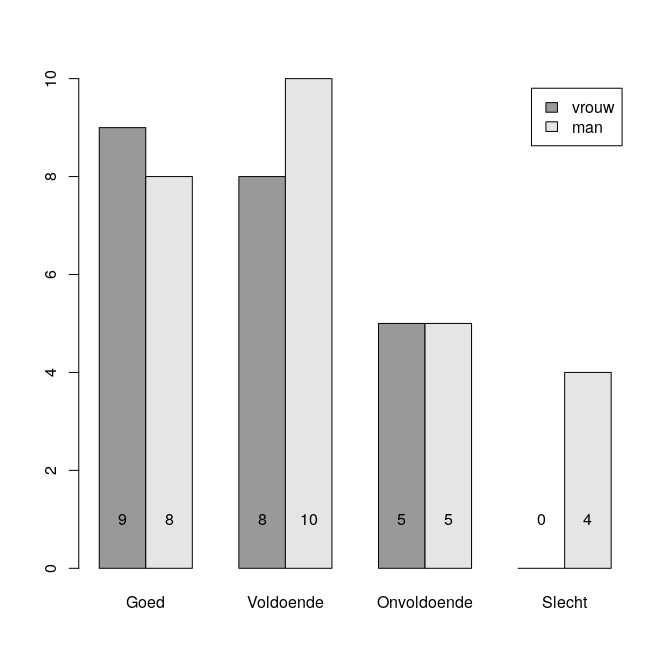
\includegraphics[height=.9\textheight]{2var-staafgrafiek-geclusterd}
  \end{figure}
  
\end{frame}

\begin{frame}
  \frametitle{Visuele voorstelling van kruistabelen}
  \framesubtitle{Rependiagram}
  
  \begin{figure}
    \centering
    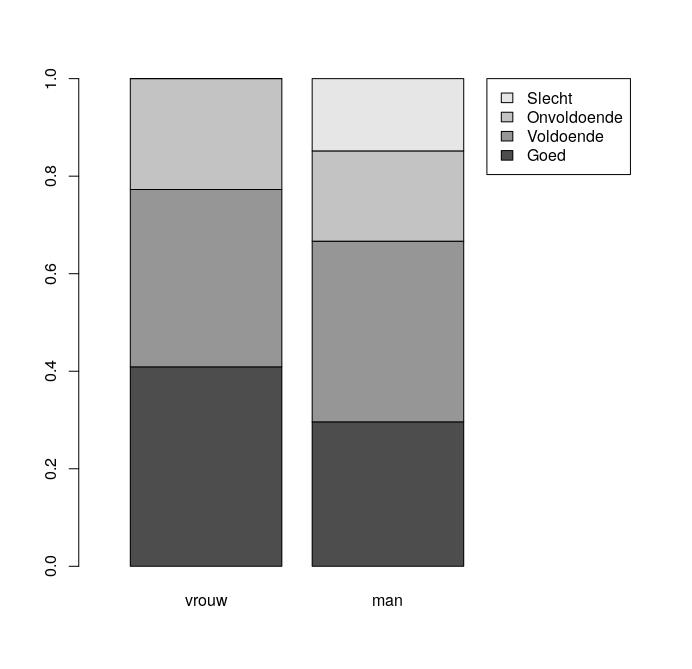
\includegraphics[height=.9\textheight]{2var-rependiagram-waardering-mv}
  \end{figure}
  
\end{frame}

\end{document}